\begin{frame}{Setup on baf}
    \begin{itemize}
        \item Create a random set of hyperparameters
        \vspace{0.2cm}
        \item Submit a job to baf for each configuration
        \vspace{0.2cm}
        \item Use dagman to wait for the jobs to finish
        \vspace{0.2cm}
        \item Evaluate the results and create the next set of configurations
        \vspace{0.2cm}
        \item \href{https://indico.desy.de/indico/event/23852/session/3/contribution/5/material/slides/0.pdf}{Anji's talk}
        \item \href{https://confluence.team.uni-bonn.de/display/PHYIT/Job+restarting+with+Dagman}{Confluence link}
    \end{itemize}
    
\end{frame}

\begin{frame}{Setup}
    \begin{itemize}
        \item \tZq as signal against \ttbar as background
        \item Using basic kinematic variables
        \item No specific region
        \item Training without weights due to some recent problems
        \item Testing: nodes, layers, dropout
        \item Fixed hyperparameters:
            \begin{itemize}
                \item Optimizer: Adam
                \item Activation: relu, sigmoid
                \item Batchsize: 1000
                \item Epochs: 25
            \end{itemize}
    \end{itemize}
\end{frame}

\begin{frame}{An example of parameter development}
     \begin{block}{Initial parameters}
         \begin{itemize}
             \item Layers: $1-10$
             \item Nodes: $1-100$
             \item Dropout: $0-1$
         \end{itemize}
     \end{block}
     \begin{block}{Final parameters}
         \begin{itemize}
             \item Layers: $4\pm2$
             \item Nodes: $67\pm33$
             \item Dropout: $0.4\pm0.3$
         \end{itemize}
     \end{block}
\end{frame}

\begin{frame}{ROC and Separation}
    \begin{columns}
        \begin{column}{0.5\textwidth}
            \begin{figure}
                \centering
                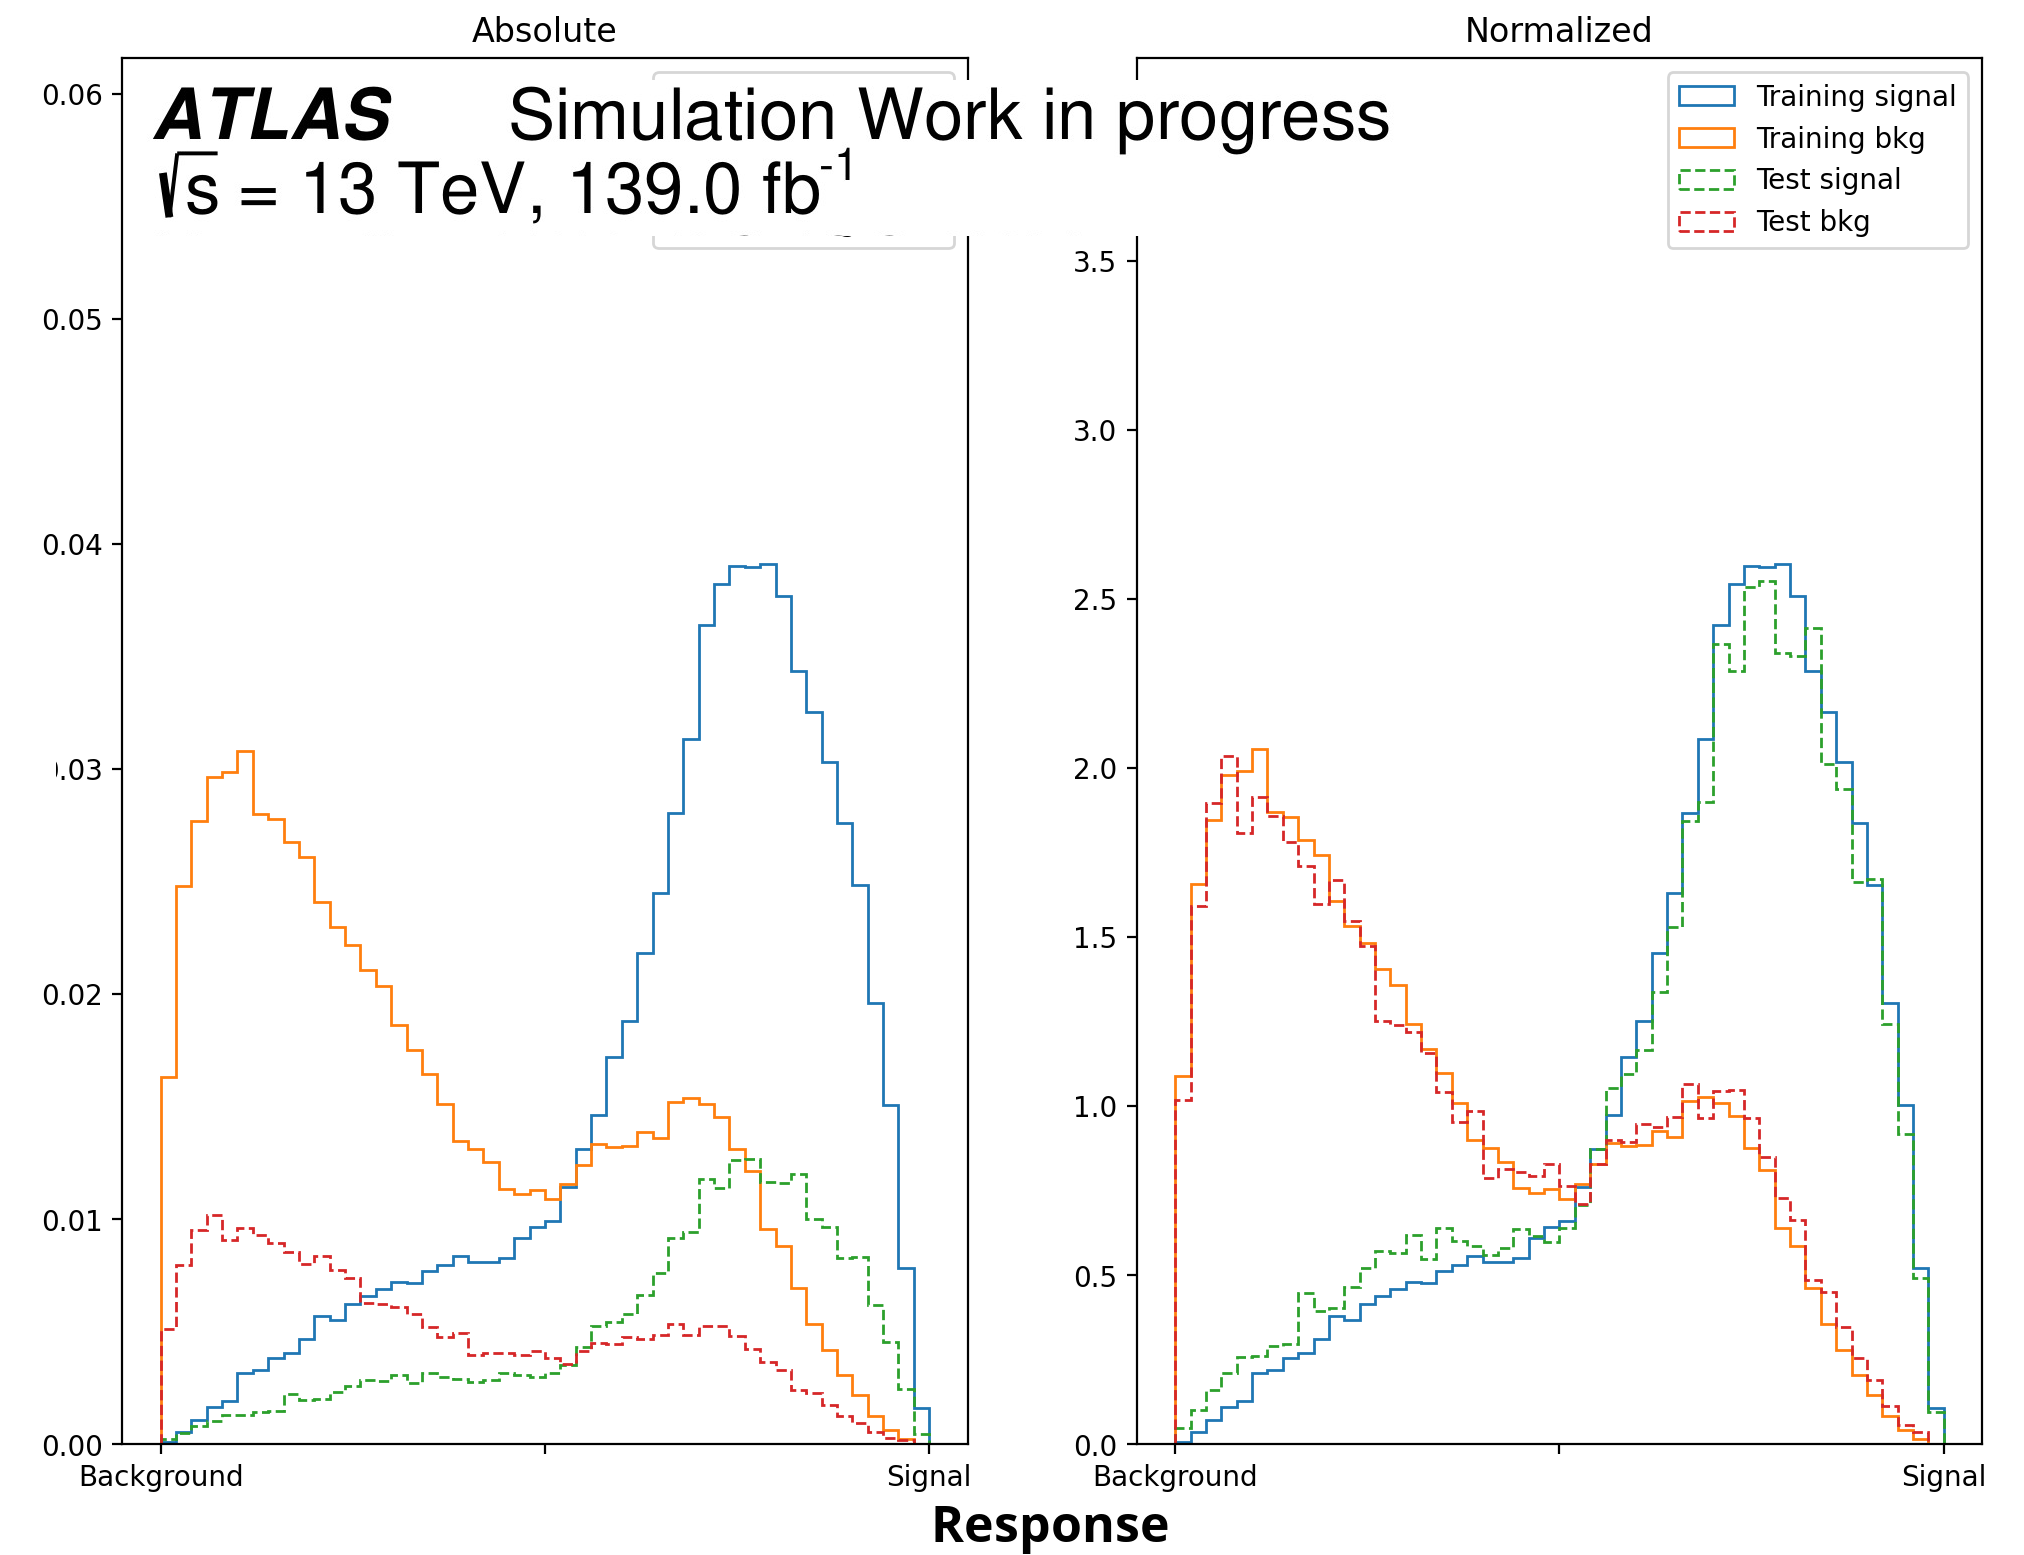
\includegraphics[width = \textwidth]{evo_response.png}
            \end{figure}
        \end{column}
        \begin{column}{0.5\textwidth}
            \begin{figure}
                \centering
                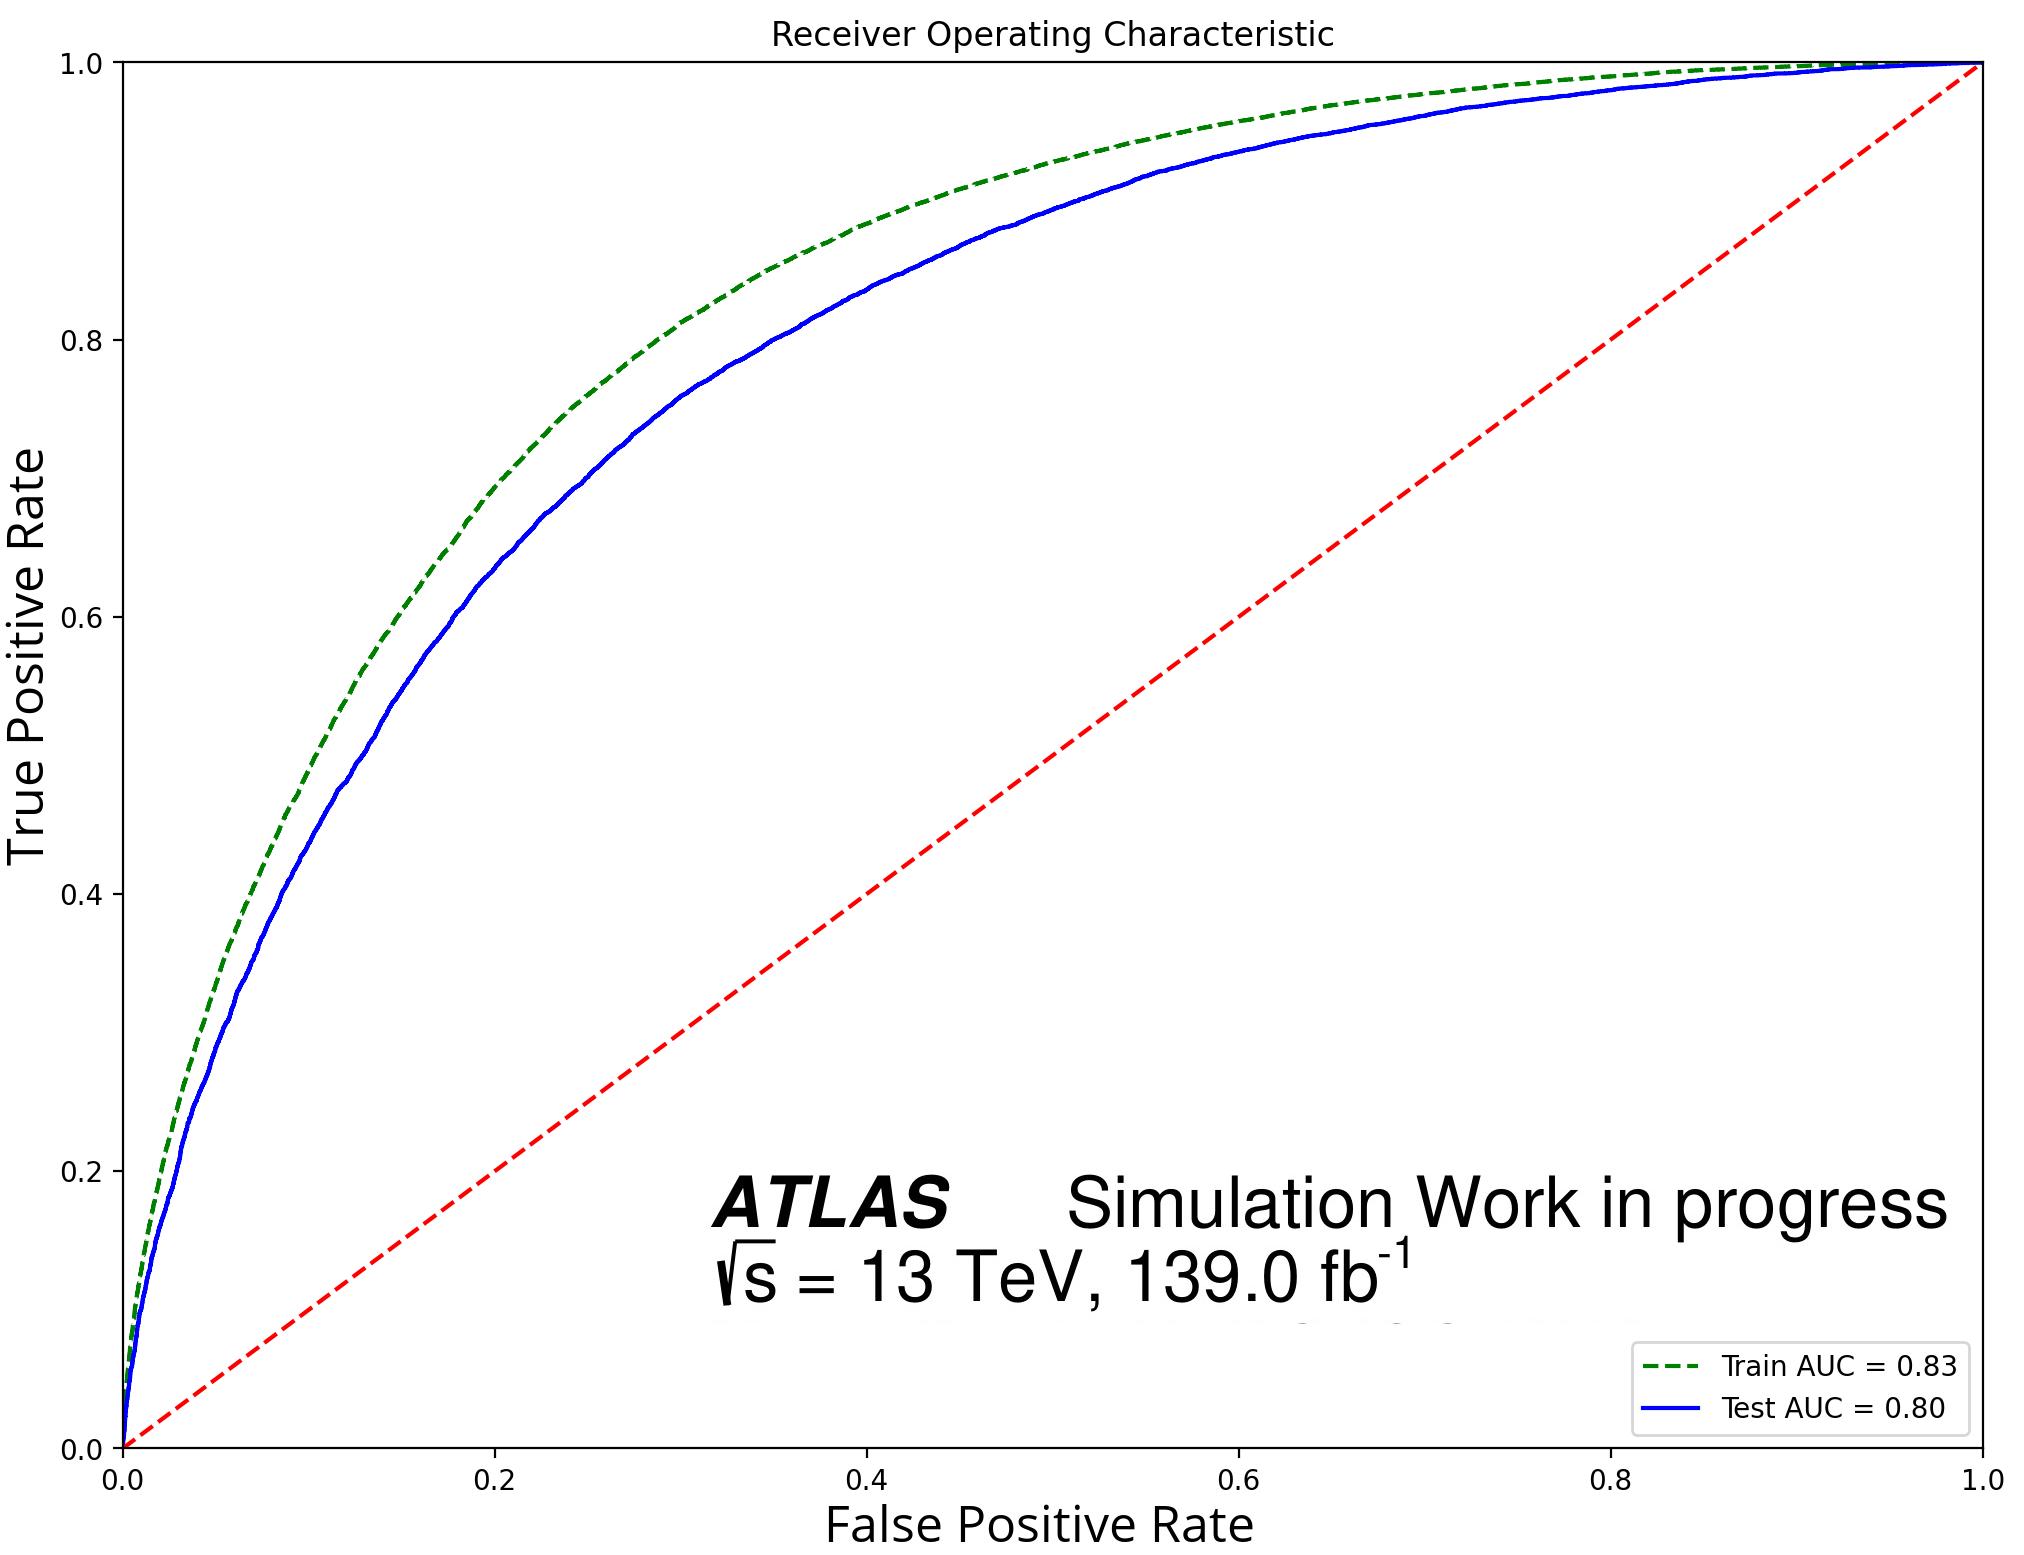
\includegraphics[width = \textwidth]{evo_ROC.png}
            \end{figure}
        \end{column}
    \end{columns}
\end{frame}

\begin{frame}{Comparing to a grid search}
    \begin{columns}
        \begin{column}{0.5\textwidth}
            \begin{figure}
                \centering
                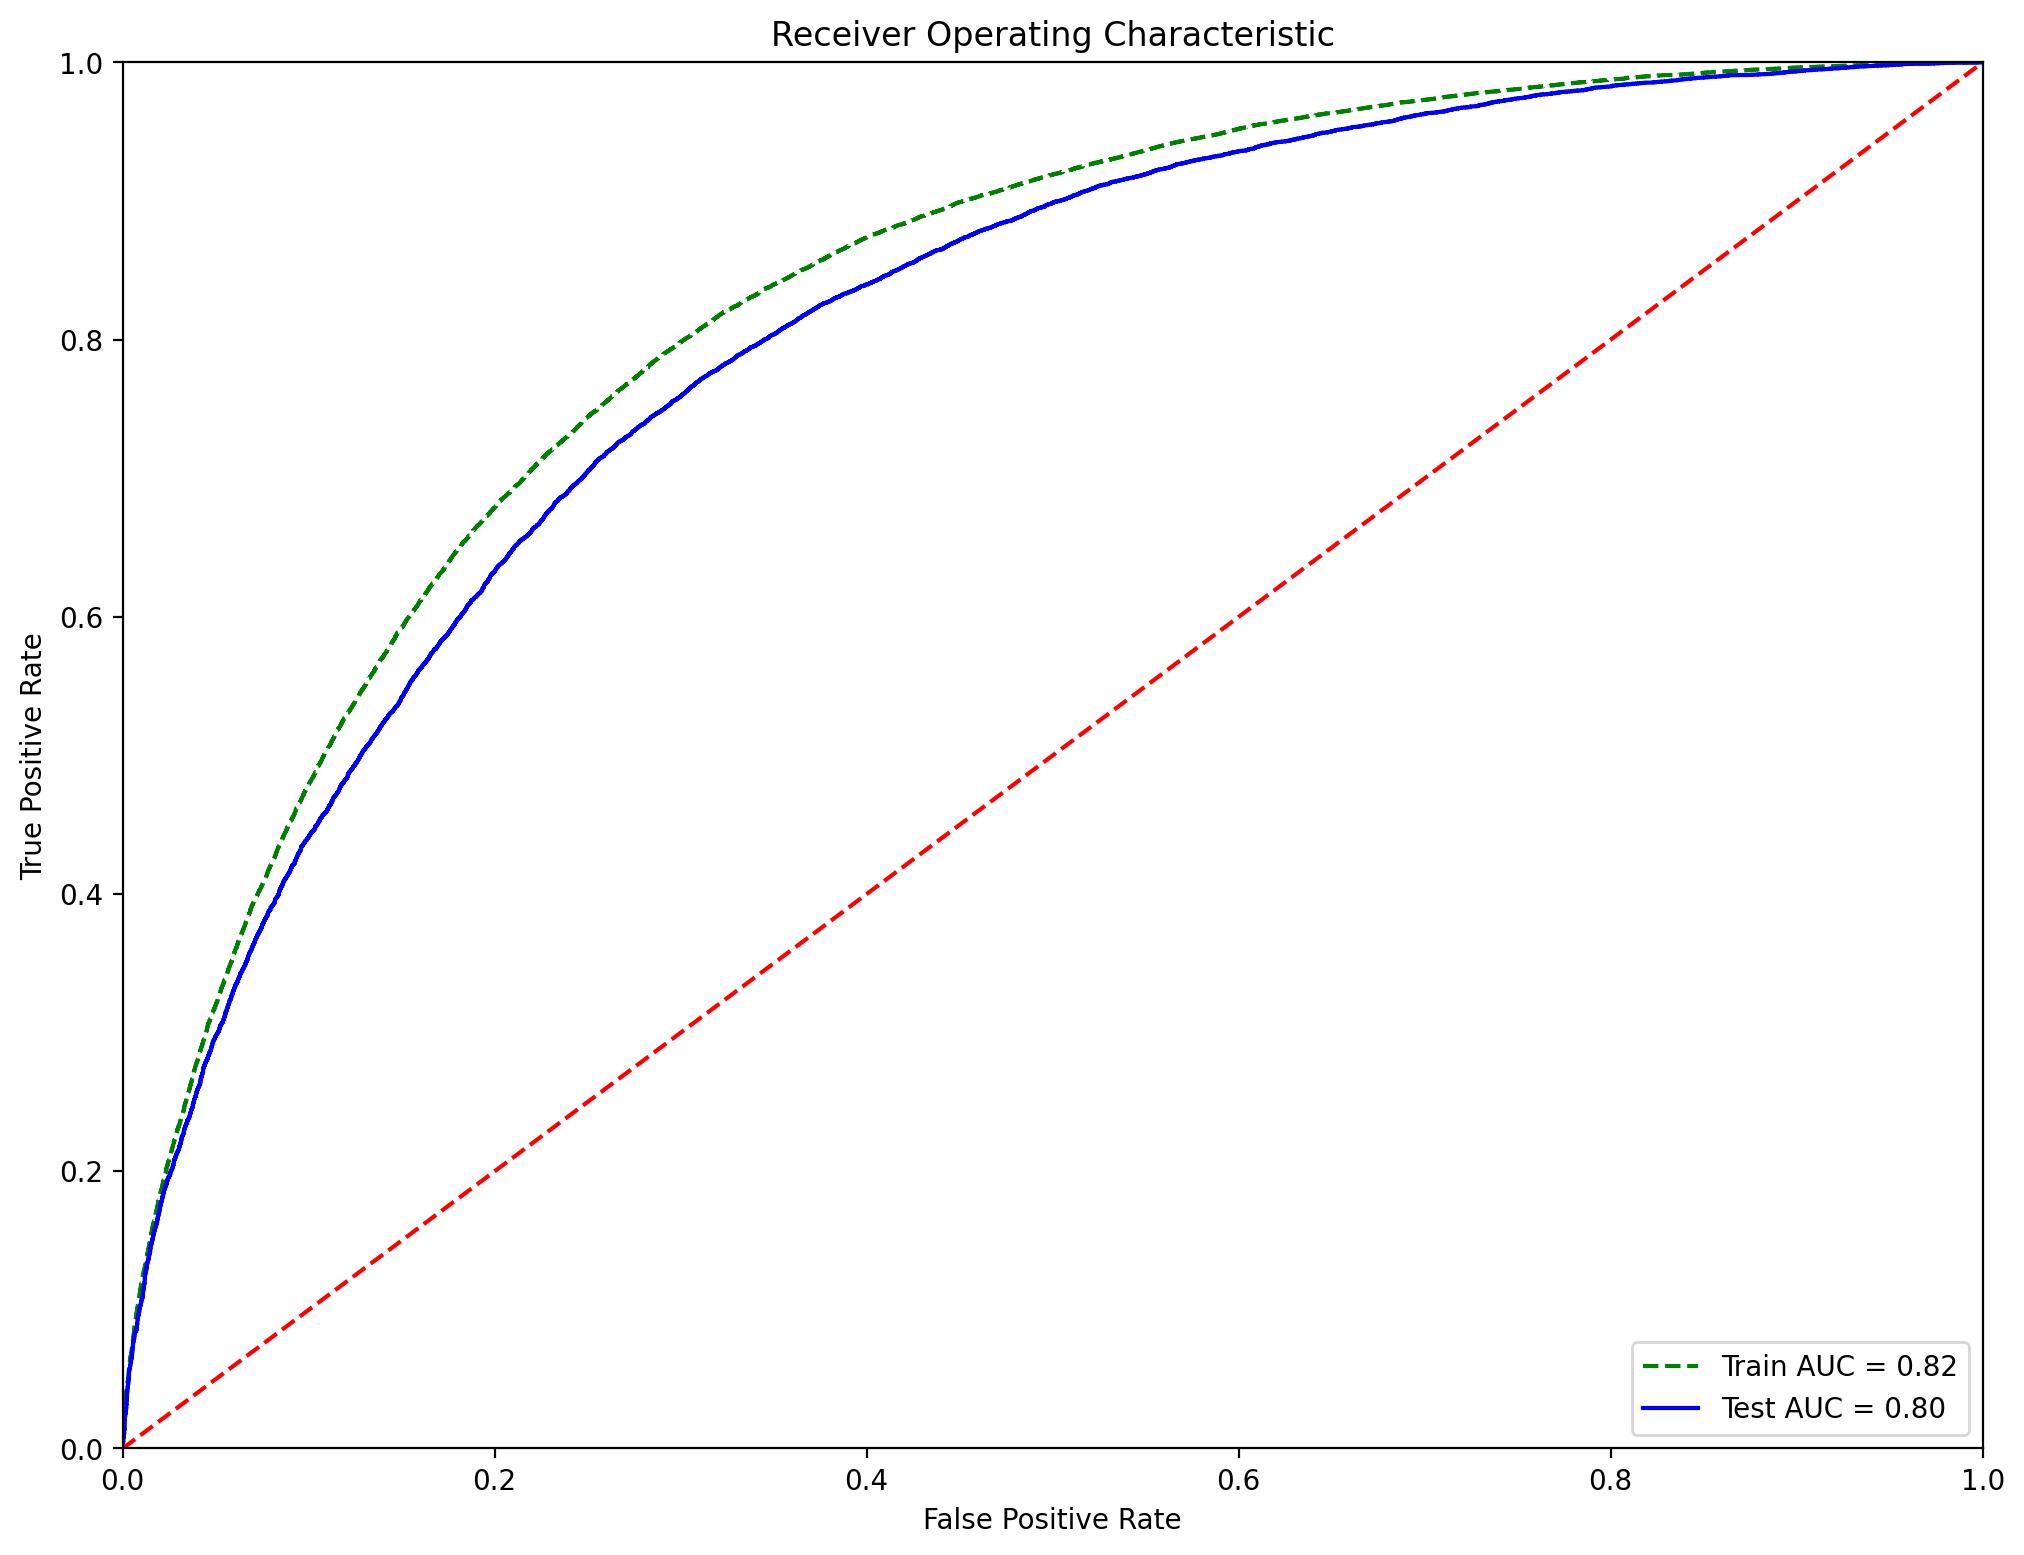
\includegraphics[width = \textwidth]{grid_ROC.png}
                \caption{Grid search}
            \end{figure}
        \end{column}
        \begin{column}{0.5\textwidth}
            \begin{figure}
                \centering
                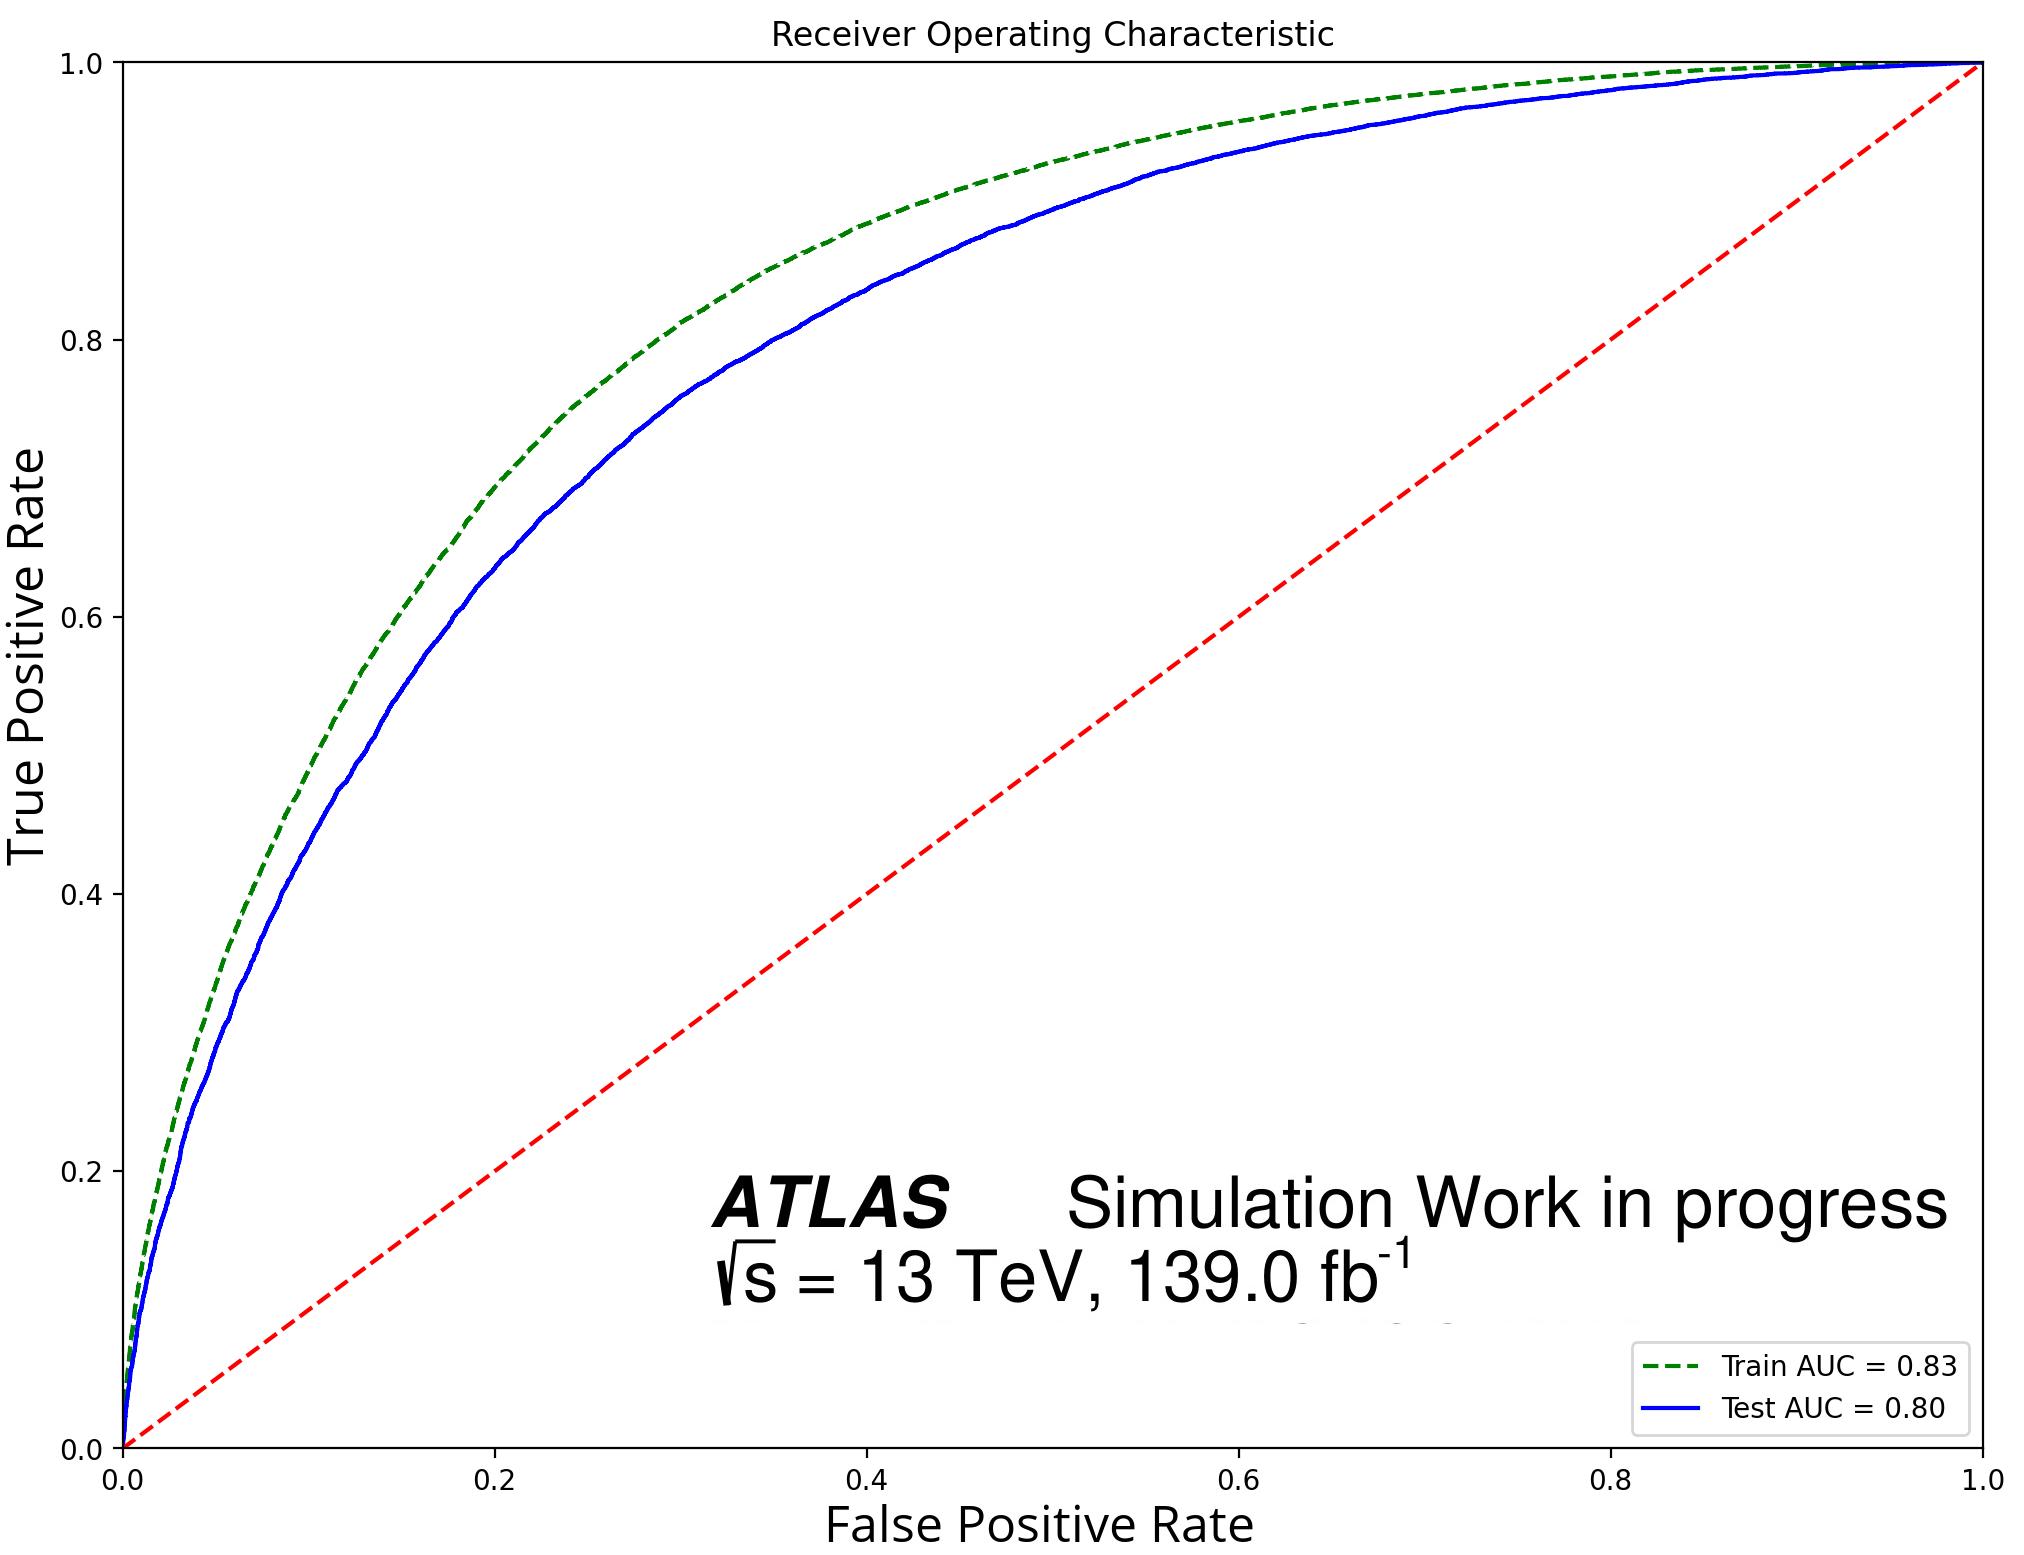
\includegraphics[width = \textwidth]{evo_ROC.png}
                \caption{Evolutionary search}
            \end{figure}
        \end{column}
    \end{columns}
\end{frame}


\begin{frame}{Comparing to a grid search}
    \begin{columns}
        \begin{column}{0.5\textwidth}
            \begin{figure}
                \centering
                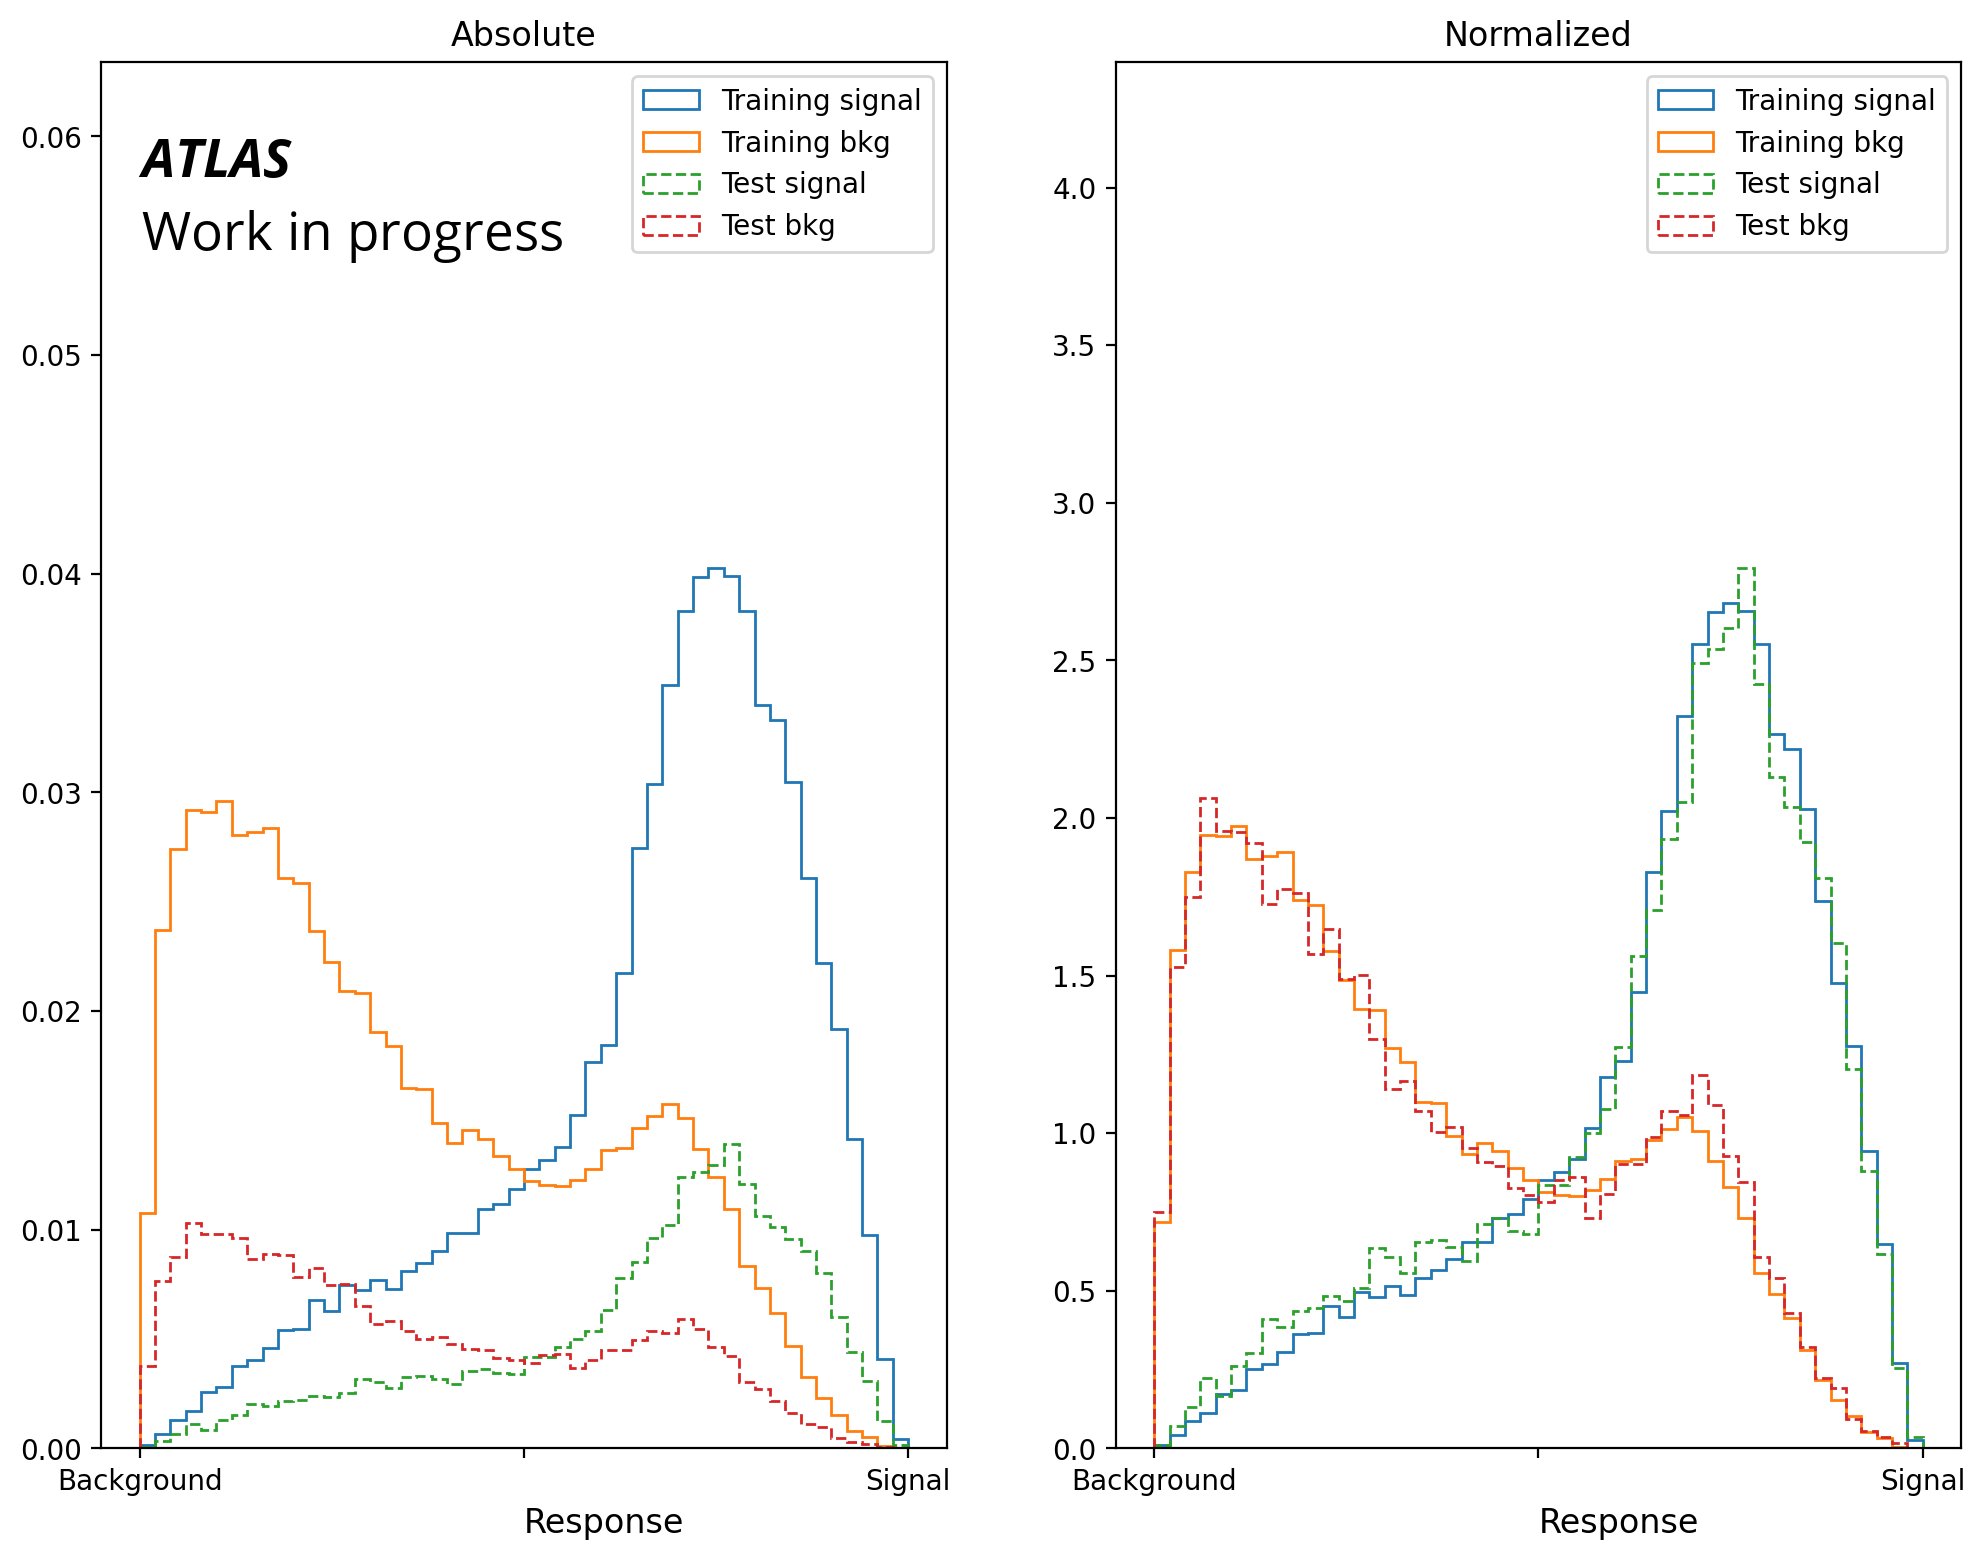
\includegraphics[width = \textwidth]{grid_response.png}
                \caption{Grid search}
            \end{figure}
        \end{column}
        \begin{column}{0.5\textwidth}
            \begin{figure}
                \centering
                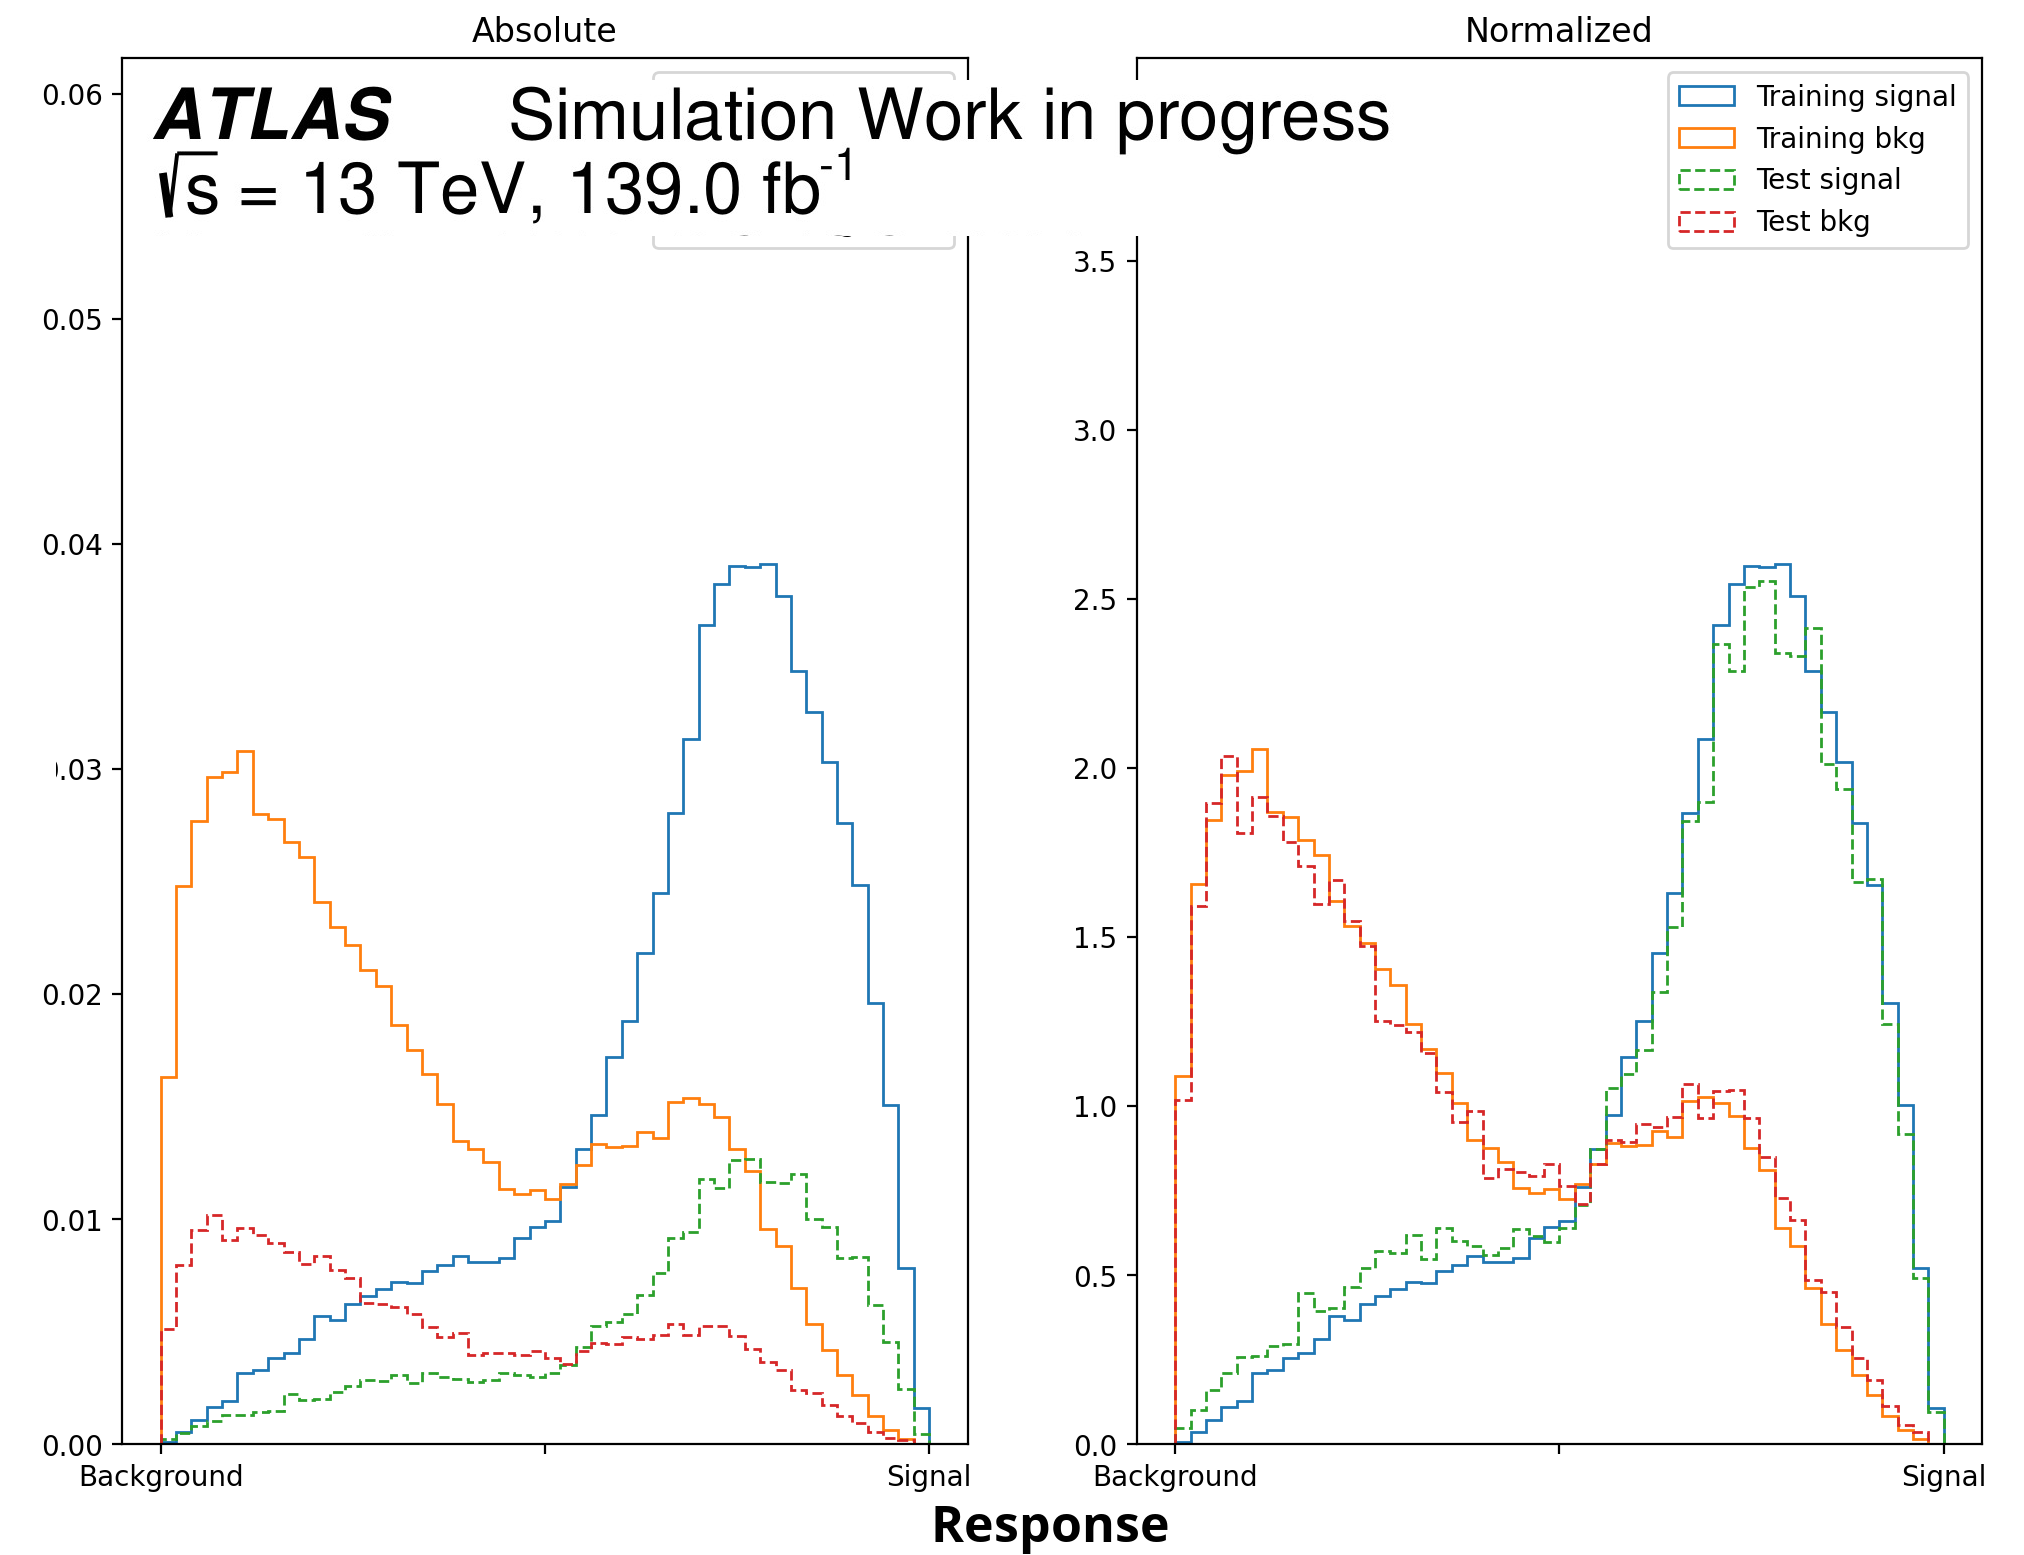
\includegraphics[width = \textwidth]{evo_response.png}
                \caption{Evolutionary search}
            \end{figure}
        \end{column}
    \end{columns}
\end{frame}